\begin{figure*}
  \centering
  \begin{tabular}{p{27mm}p{27mm}p{27mm}p{27mm}p{27mm}}
    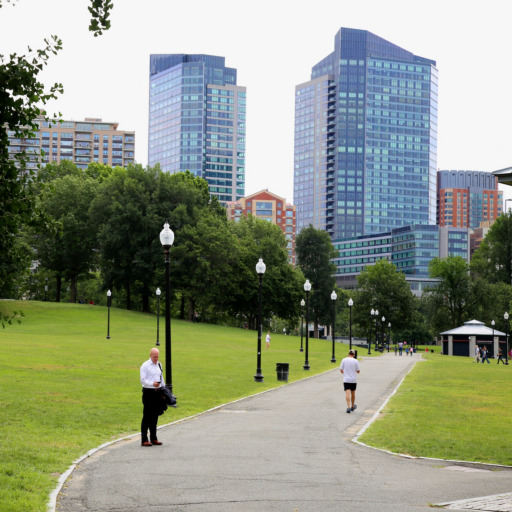
\includegraphics[width=30mm]{figs/inpaint/15_orig} &
    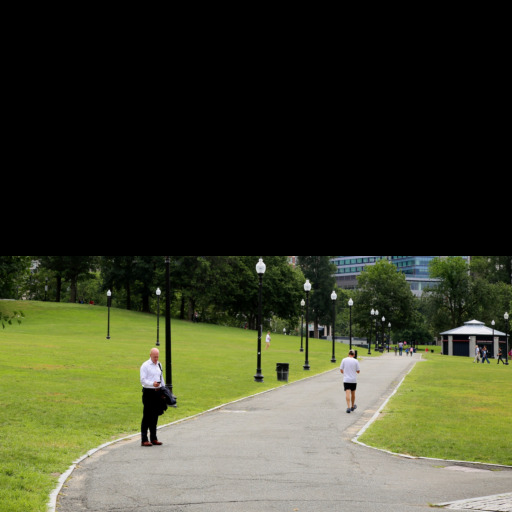
\includegraphics[width=30mm]{figs/inpaint/15_masked} &
    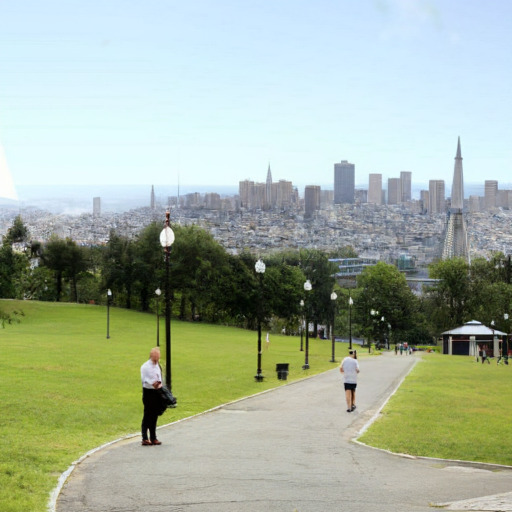
\includegraphics[width=30mm]{figs/inpaint/14_synth_07} &
    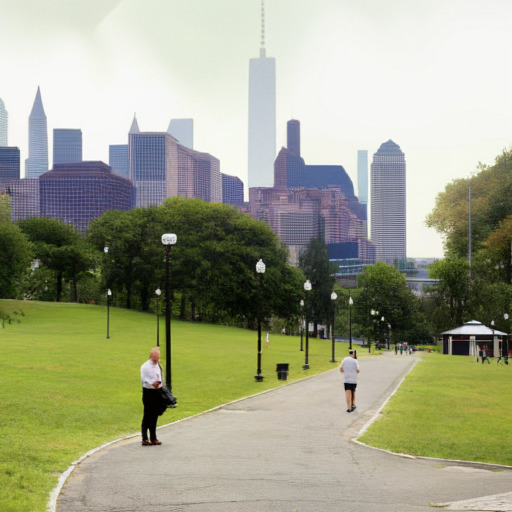
\includegraphics[width=30mm]{figs/inpaint/12_synth_00} &
    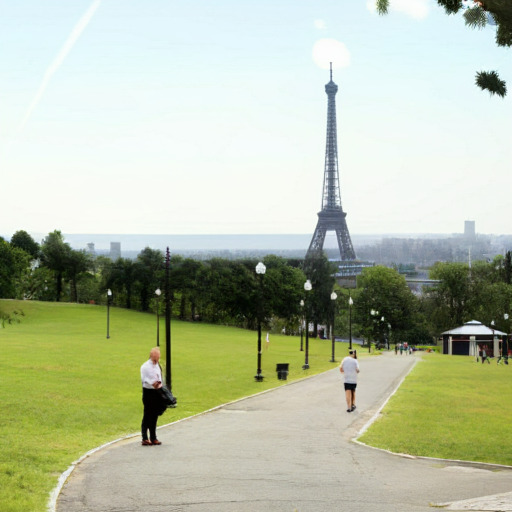
\includegraphics[width=30mm]{figs/inpaint/15_synth_07} 
    \\
     Original &
     Masked &
    {San Francisco in the background} & 
    {New York City in the background} &
    {Paris in the background} 
    \\
    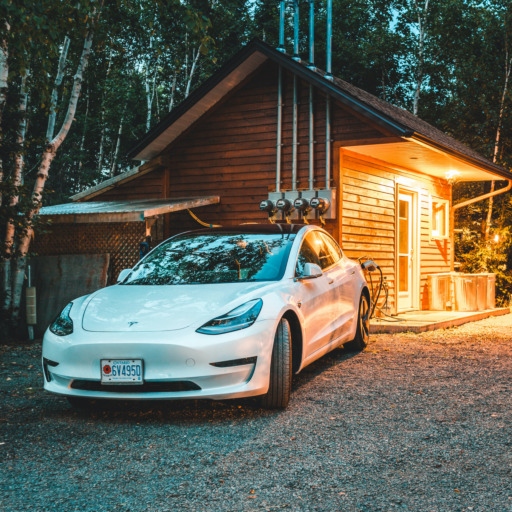
\includegraphics[width=30mm]{figs/inpaint/17_orig} &
    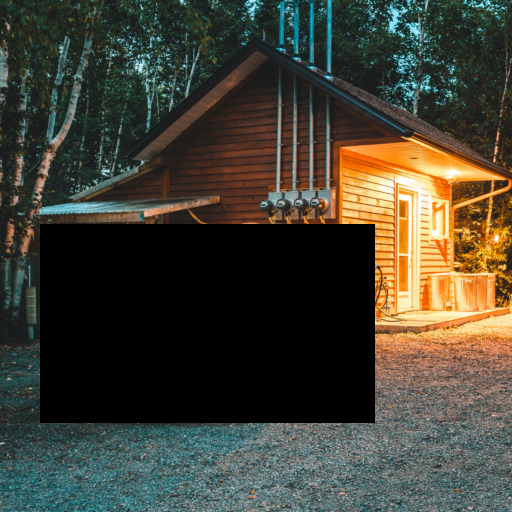
\includegraphics[width=30mm]{figs/inpaint/18_masked} &
    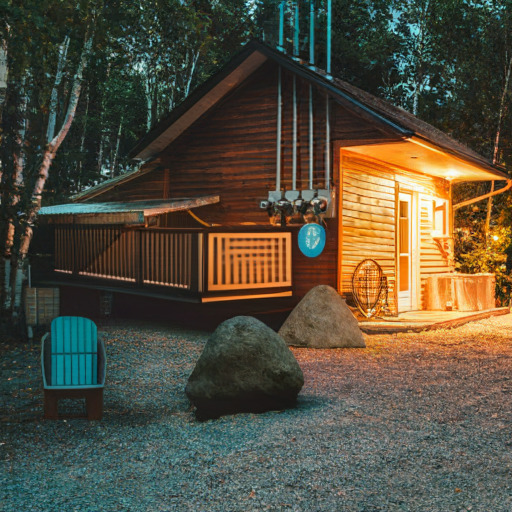
\includegraphics[width=30mm]{figs/inpaint/18_synth_07} &
    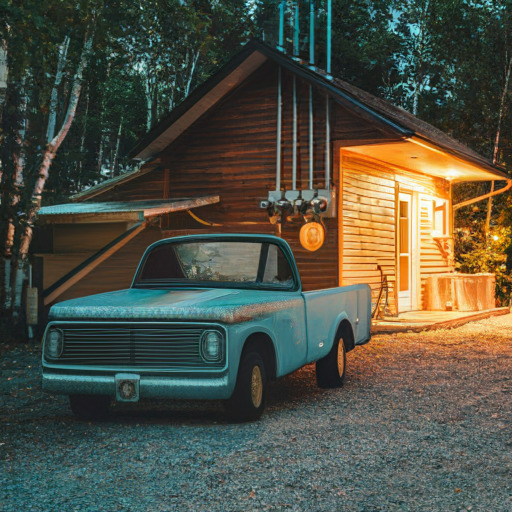
\includegraphics[width=30mm]{figs/inpaint/old_pickup} &
    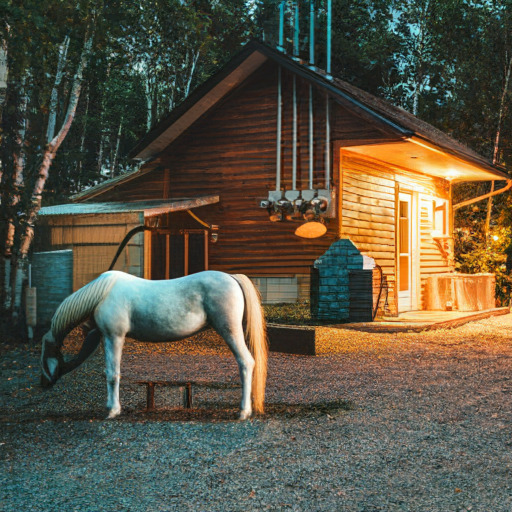
\includegraphics[width=30mm]{figs/inpaint/horse} 
    \\
    Original &
    Masked &
    {A cabin in the woods} & 
    {An old, beat up pickup truck.} & 
    {A horse tied to a post.} 
  \end{tabular}
  \caption{\small Examples of text-guided inpainting. The mask is shown in the second column of each row. This behavior arises directly from the model with no fine-tuning.}
  %\vspace{-30pt}
  \label{fig:inpainting}
\end{figure*}